\documentclass[aspectratio=169]{beamer}

\usetheme{default}
\usefonttheme{professionalfonts}
\setbeamertemplate{navigation symbols}{}
\setbeamertemplate{itemize items}[circle]
\setbeamercolor{itemize item}{fg=white}

\setbeamerfont{title}{series=\bfseries, size=\normalfont\Large}
\setbeamercolor{title}{fg=white}

\setbeamerfont{author}{size=\normalfont\small}
\setbeamercolor{author}{fg=white}

\setbeamerfont{frametitle}{series=\bfseries, size=\normalfont}
\setbeamercolor{frametitle}{fg=white}

\setbeamerfont{framesubtitle}{size=\normalfont\large}
\setbeamercolor{framesubtitle}{fg=white}

\setbeamercolor{background canvas}{bg=black}
\setbeamercolor{normal text}{fg=white}

\usepackage[utf8]{inputenc}
\usepackage[french]{babel}
\usepackage{amsmath}
\usepackage{amsfonts}
\usepackage{amssymb}
\usepackage{graphicx}
\usepackage[]{bm}
\usepackage[]{multimedia}
\usepackage[]{multicol}
\usepackage[squaren,Gray]{SIunits}

\graphicspath{{imgs/}}

\usepackage{tikz} % Required for drawing custom shapes
\usetikzlibrary{arrows}
\usetikzlibrary{shapes.geometric, math, positioning, calc, patterns, angles, quotes}
\usetikzlibrary{patterns.meta,decorations.pathmorphing}




\usepackage[]{listings}

\definecolor{codegreen}{rgb}{0,0.8,0}
\definecolor{codegray}{rgb}{0.5,0.5,0.5}
%\definecolor{codepurple}{rgb}{0.58,0,0.82}
\definecolor{codepurple}{rgb}{0,0.8,0}
\definecolor{backcolour}{rgb}{0.0, 0.0, 0.0}

\lstdefinestyle{mystyle}{
  backgroundcolor=\color{backcolour},
  commentstyle=\color{codegreen},
  keywordstyle=\color{magenta},
  numberstyle=\tiny\color{codegray},
  stringstyle=\color{codepurple},
  basicstyle=\ttfamily\footnotesize,
  breakatwhitespace=false,
  breaklines=true,
  captionpos=b,
  keepspaces=true,
  numbers=left,
  numbersep=5pt,
  showspaces=false,
  showstringspaces=false,
  showtabs=false,
  tabsize=2
}

\lstset{style=mystyle}



\title{Introduction à Python}
\author{Jean-Christophe LOISEAU}
\institute{Arts \& Métiers Institute of Technology, 2021-2022}
\date{}

\begin{document}





\frame{\titlepage}





\begin{frame}
  \begin{minipage}{.64\textwidth}
    \textbf{\alert{NumPy}} : bibliothèque (ou package) pour \textbf{Python} destinée à manipuler des \textbf{matrices} ou \textbf{tableaux multidimensionels} ainsi que des fonctions mathématiques opérant sur ces tableaux.
  \end{minipage}%
  \hfill
  \begin{minipage}{.32\textwidth}
    \centering
    
\includegraphics[width=\textwidth]{numpy_logo}
  \end{minipage}

  \vspace{-1cm}
\end{frame}





\begin{frame}
  \vfill
  \centering
  
\includegraphics[width=.16\textwidth]{fortran_logo}%
  \hfill
  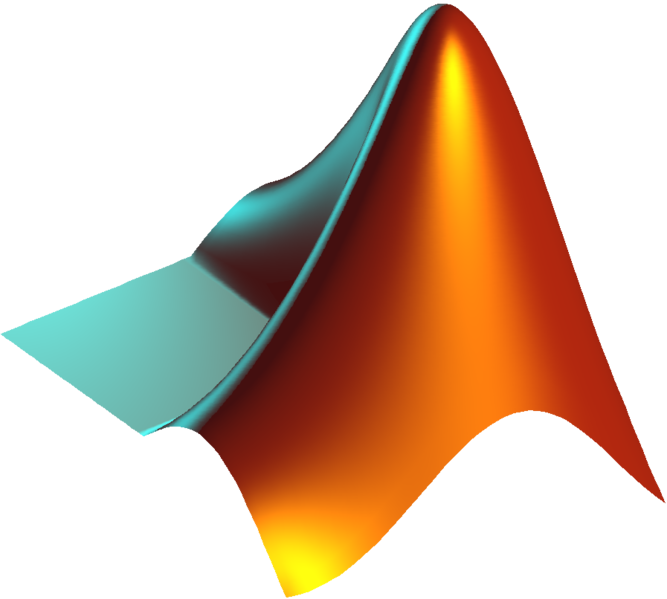
\includegraphics[width=.16\textwidth]{matlab_logo}%
  \hfill
  
\includegraphics[width=.16\textwidth]{octave_logo}%
  \hfill
  
\includegraphics[width=.24\textwidth]{julia_logo}
  \vfill
\end{frame}





\begin{frame}
\end{frame}



\begin{frame}[fragile]{}{}
  \begin{lstlisting}[language=Python]
    def matvec(A, x):
        m, n = len(A), len(A[0])
        b = [sum(A[i][j]*x[j] for j in range(n)) for i in range(m)]
        return b


    b = matvec(A, x)
  \end{lstlisting}
  \vspace{-1.5cm}
\end{frame}




\begin{frame}[fragile]{}{}
  \begin{lstlisting}[language=Python]
    import numpy as np

    b = A @ x
  \end{lstlisting}

  \vspace{-1.5cm}
\end{frame}




\begin{frame}
  \vfill
  \centering
  Performances pour une matrice $\bm{A}$ de taille $10 \times 10$.

  \bigskip

  \begin{tabular}{l|ccc}
    ~ & Addition & Transposition & Produit matrice-vecteur \\
    \hline

    \textbf{Python} & \unit{15.2}{\micro\second} & \unit{10}{\micro\second} & \unit{14.9}{\micro\second} \\
    \textbf{NumPy} & \unit{0.5}{\micro\second}  & \unit{0.1}{\micro\second} & \unit{1.2}{\micro\second}
  \end{tabular}
  \vfill
\end{frame}




\begin{frame}
  \vfill
  \centering
  Performances pour une matrice $\bm{A}$ de taille $1000 \times 1000$.

  \bigskip

  \begin{tabular}{l|ccc}
    ~ & Addition & Transposition & Produit matrice-vecteur \\
    \hline

    \textbf{Python} & \unit{0.136}{\second} & \unit{0.111}{\second} & \unit{0.1}{\second} \\
    \textbf{NumPy} & \unit{2.5}{\milli\second}  & \unit{0.15}{\micro\second} & \unit{0.5}{\milli\second}
  \end{tabular}
  \vfill
\end{frame}





\begin{frame}[fragile]{}{}
  \vfill
  \begin{lstlisting}[language=Python]
    x = [1, 2]
    # [1, 2]

    x.append('Je suis du texte')
    # [1, 2, 'Je suis du texte']

    x.extend([4, 5])
    # [1, 2, 'Je suis du texte', 4, 5]

    y = ['Encore du texte', 8]
    z = x + y
    # [1, 2, 'Je suis du texte', 4, 5, 'Encore du texte', 8]
  \end{lstlisting}
  \vfill
\end{frame}





\begin{frame}[fragile]{}{}
  
\end{frame}





\begin{frame}[fragile]{}{}
  \vfill
  \begin{lstlisting}[language=Python]
    import numpy as np

    x = np.array([1, 2])
    # array([1, 2])

    y = x + np.array([4, 5])
    # array([5, 7])

    z = x + np.array([4, 5, 6])
    # Affiche une erreur !
  \end{lstlisting}
  \vfill
\end{frame}




\begin{frame}[fragile]{}{}

\end{frame}




\begin{frame}[fragile]{}{}
  \vfill
  \begin{lstlisting}[language=Python]
    np.array(object, dtype=None, ndim=0)
  \end{lstlisting}
  %
  \begin{itemize}
  \item \texttt{object} : Typiquement une liste de nombres pour un vecteur, ou une liste de liste de nombres pour une matrice.

  \item \texttt{dtype} : Le type choisi pour le stockage des données (optionnel).
  \end{itemize}
  \vfill
\end{frame}

\begin{frame}
  \begin{multicols}{2}
    \begin{itemize}
    \item \texttt{np.bool} : Booléen (\texttt{True} ou \texttt{False})

    \item \texttt{np.int8} : Entier ($-128$ à $127$)
    \item \texttt{np.int16} : Entier ($-2^{15}$ à $2^{15}-1$)
    \item \texttt{np.int32} : Entier ($-2^{31}$ à $2^{31}-1$)
    \item \texttt{np.int64} : Entier ($-2^{63}$ à $2^{63}-1$)

    \item \texttt{np.uint8} : Entier ($0$ à $255$)
    \item \texttt{np.unint16} : Entier ($0$ à $2^{16}-1$)
    \item \texttt{np.unint32} : Entier ($0$ à $2^{32}-1$)
    \item \texttt{np.unint64} : Entier ($0$ à $2^{64}-1$)

    \item \texttt{np.float16} : Flottant (demi-précision)
    \item \texttt{np.float32} : Flottant (simple précision)
    \item \texttt{np.float64} : Flottant (double précision)

    \item \texttt{np.complex64} : Complexe (simple précision)
    \item \texttt{np.complex128} : Complexe (double précision)
    \end{itemize}
  \end{multicols}
\end{frame}




\begin{frame}[fragile]{}{}
  \vfill
  \begin{lstlisting}[language=Python]
    x = np.array([1, 2, 3])
    x.dtype
    # dtype('int64')

    x = np.array([1.0, 2, 3])
    x.dtype
    # dtype('float64')

    x = np.array([1, 2, 3], dtype=np.float32)
    x.dtype
    # dtype('float32')
  \end{lstlisting}
  \vfill
\end{frame}




\begin{frame}[fragile]{}{}
  \vfill
  \begin{lstlisting}[language=Python]
    x = np.array([1, 2, 3])
    x.shape
    # (3,)

    x = np.array([[1, 2, 3]])
    x.shape
    # (1, 3)

    x = np.array([[1], [2], [3]])
    x.shape
    # (3, 1)
  \end{lstlisting}
  \vfill
\end{frame}





\begin{frame}[fragile]{}{}
  \vfill
  \begin{minipage}{.60\textwidth}
    \begin{lstlisting}[language=Python]
      A = np.array([[1, 2], [4, 5]])
      # array([[1, 2],
      #        [3, 4]])
      
      A.dtype
      # dtype('int64')
      
      A.shape
      # (2, 2)
    \end{lstlisting}
  \end{minipage}%
  \hfill
  \begin{minipage}{.36\textwidth}
    \begin{lstlisting}[language=Python]
      A[0, 0]
      # 1

      A[0] # ou A[0, :]
      # array([1, 2])

      A[:, 0]
      # array([1, 3])
    \end{lstlisting}
  \end{minipage}
  \vfill
\end{frame}




\begin{frame}[fragile]{}{}
  \vfill
  \begin{lstlisting}[language=Python]
    z = 1 + 1j * 2
    # z = 1 + 2i

    z = np.array([1.0, 2 + 1j*100])
    # z = [1 , 2 + 100i]

    z.real
    # [1 , 2]

    z.imag
    # [0 , 100]

    z.conj()
    # [1 , 2 - 100i]
  \end{lstlisting}
  \vfill
\end{frame}




\begin{frame}
  \vfill
  \centering
  \textbf{Opérations sur des arrays numpy}
  \vfill
\end{frame}




\begin{frame}[fragile]{}{}
  \vfill
  \begin{itemize}
  \item Création d'un array de 0 : \verb+np.zeros((d0, d1, ..., dn), dtype=None)+
    %
    \begin{lstlisting}[language=Python]
      x = np.zeros(10)
      x = np.zeros((4, 3), dtype=np.int32)
      x = np.zeros((2, 4, 10), dtype=np.complex128)
    \end{lstlisting}

  \item Création d'un array de 1 : \verb+np.ones((d0, d1, ..., dn), dtype=None)+
    %
    \begin{lstlisting}[language=Python]
      x = np.ones(10)
      x = np.ones((4, 3), dtype=np.int32)
      x = np.ones((2, 4, 10), dtype=np.complex128)
    \end{lstlisting}
  \end{itemize}
  \vfill
\end{frame}




\begin{frame}[fragile]{}{}
  \vfill
  \begin{minipage}{.48\textwidth}
    \begin{lstlisting}[language=Python]
      x = np.array([1, 2, 3])

      x.sum()     # np.sum(x)
      # 6
      
      x.prod()    # np.prod(x)
      # 6
      
      x.mean()    # np.mean(x)
      # 2
      
      x.std()     # np.std(x)
      # 0.81649
    \end{lstlisting}
  \end{minipage}%
  \hfill
  \begin{minipage}{.48\textwidth}
    \begin{lstlisting}[language=Python]
      x.max()    # np.max(x)
      # 3
      
      x.min()    # np.min(x)
      # 1
      
      x.argmax() # np.argmax(x)
      # 2
      
      x.argmin() # np.argmin(x)
      # 0

      x.abs() # np.abs(x)
    \end{lstlisting}
  \end{minipage}
  \vfill
\end{frame}





\begin{frame}[fragile]{}{}
  \vfill
  \begin{lstlisting}[language=Python]
    A = np.array([[1, 2], [3, 4]])
    # array([[1, 2],
    #        [3, 4]])
    
    A.sum()           # np.sum(A)
    # 10
    
    A.sum(axis=0)     # np.sum(A, axis=0)
    # array([4, 6])
    
    A.sum(axis=1)     # np.sum(A, axis=1)
    # array([3, 7])

    A.T               # np.transpose(A)
    # array([[1, 3],
    #        [2, 4]])
  \end{lstlisting}
  \vfill
\end{frame}




\begin{frame}[fragile]{}{}
  \vfill
  \begin{minipage}{.48\textwidth}
    \begin{lstlisting}[language=Python]
      y = np.exp(x)
      
      y = np.cos(x)
      
      y = np.sin(x)
      
      y = np.tan(x)
      
      y = np.cosh(x)
      
      y = np.sinh(x)
    \end{lstlisting}
  \end{minipage}%
  \hfill
  \begin{minipage}{.48\textwidth}
    \begin{lstlisting}[language=Python]
      y = np.log(x)

      y = np.arccos(x)
      
      y = np.arcsin(x)
      
      y = np.arctan(x)
      
      y = np.arccosh(x)
      
      y = np.arcsinh(x)
    \end{lstlisting}
  \end{minipage}
  \vfill
\end{frame}




\begin{frame}[fragile]{}{}
  \vfill
  \begin{itemize}
  \item \textbf{\alert{np.linalg}} : Méthodes de base pour l'algèbre linéaire (e.g.\ inversion de matrice, résolution de système linéaire, valeurs propres, etc).

    \bigskip

  \item \textbf{\alert{np.random}} : Génération de nombres aléatoires provenant de différentes distributions (e.g.\ normale, Laplace, Gamma, etc).

    \bigskip

  \item \textbf{\alert{np.fft}} : Transformées de Fourier rapides (1D, 2D et nD) utiles pour le traitement du signal et des images.
  \end{itemize}
  \vfill
\end{frame}

\begin{frame}[fragile]{}{}
  \vfill
  \begin{lstlisting}[language=Python]
    import numpy as np
    import numpy.linalg as npl
  \end{lstlisting}
  \vfill
\end{frame}

\begin{frame}[fragile]{}{}
  \vfill
  \begin{lstlisting}[language=Python]
    x, y = np.array([1, 2]), np.array([3, 4])

    # Produit scalaire.
    c = np.vdot(x, y)

    # Norme Euclidienne.
    c = npl.norm(x)
  \end{lstlisting}
  \vfill
\end{frame}

\begin{frame}[fragile]{}{}
  \vfill
  \begin{lstlisting}[language=Python]
    A = np.array([[1, 2], [3, 4]])

    # Inverse.
    B = npl.inv(A)

    # Determinant.
    d = npl.det(A)

    # Valeurs propres et vecteurs propres.
    vals, vecs = npl.eig(A)     # vals = npl.eigvals(A)

    # Elevation d'une matrice A a la puissance k .
    B = npl.matrix_power(A, k)
  \end{lstlisting}
  \vfill
\end{frame}

\begin{frame}[fragile]{}{}
  \vfill
  \begin{lstlisting}[language=Python]
    # Produit matrice-matrice / matrice-vecteur.
    y = A @ x     # np.dot(A, x)     A.dot(x)     npl.matmul(A, x)

    # Resolution de systeme lineaire.
    x = npl.solve(A, b)

    # Resolution au sens des moindres-carres.
    x = npl.lstsq(A, b)
  \end{lstlisting}
  \vfill
\end{frame}





\begin{frame}[fragile]{}{}
  \centering

  \[
  \textrm{Résoudre} \quad \bm{Ax} = \bm{b} \quad \textrm{numériquement}.
  \]

  \bigskip

  \begin{minipage}{.4\textwidth}
    \begin{lstlisting}[language=Python]
      x = npl.inv(A) @ b
    \end{lstlisting}
  \end{minipage}%
  \hfill
  \begin{minipage}{.2\textwidth}
    \centering
    ou
  \end{minipage}%
  \hfill
  \begin{minipage}{.4\textwidth}
    \begin{lstlisting}[language=Python]
      x = npl.solve(A, b)
    \end{lstlisting}
  \end{minipage}
\end{frame}







\begin{frame}[fragile]{}{}
  \vfill
  \begin{lstlisting}[language=Python]
    import numpy as np
    import numpy.random as npr
  \end{lstlisting}
  \vfill
\end{frame}

\begin{frame}[fragile]{}{}
  \vfill
  \begin{lstlisting}[language=Python]
    # Genere n nombres aleatoires issus d'une distribution normale.
    x = npr.normal(loc=0.0, size=1.0, size=n)

    # Genere n nombres aleatoires issus d'une distribution uniforme.
    x = npr.uniform(low=0.0, high=1.0, size=n)


    import matplotlib.pyplot as plt
    plt.hist(x)
  \end{lstlisting}
  \vfill
\end{frame}


\begin{frame}[fragile]{}{}
  \vfill
  \begin{lstlisting}[language=Python]
    # Sauvegarde un array en format texte.
    np.savetxt('mon_fichier.dat', x)

    # Charge un array a partir d'un fichier texte.
    x = np.loadtxt('mon_fichier.dat')
  \end{lstlisting}
  \vfill
\end{frame}

\begin{frame}
  \centering

  
\includegraphics[width=.5\textwidth]{numpy_logo}

  Pour en savoir plus, rendez-vous sur \url{https://numpy.org/}
\end{frame}

\end{document}
